\documentclass{article}

% Language
\newcommand{\mylanguage}{english}
\usepackage[T1]{fontenc}
\usepackage[\mylanguage]{babel}
\selectlanguage{\mylanguage}

% Math & figures
\usepackage{amsmath}
\usepackage{amssymb}
\usepackage{tikz}
\usepackage{graphicx}

% Hyperlinks
\usepackage{hyperref}

% FHJ mandatory setting

% Bibliography
\usepackage[
  backend=biber,
  style=numeric,
  natbib=true,
  hyperref=true,
]{biblatex}
\addbibresource{literature.bib}

% Title information (FHJ style)
\title{Overfitting vs. Underfitting in Machine Learning}



\begin{document}

\maketitle

\begin{abstract}
Overfitting and underfitting are two fundamental challenges in machine learning
that directly affect a model's ability to generalize to unseen data. This paper
explains both phenomena, their causes, consequences, and common mitigation
strategies. Mathematical formulations and graphical illustrations are used to
provide an intuitive understanding of the bias--variance trade-off.
\end{abstract}

\section{Introduction}
\label{sec:introduction}

Machine learning models aim to learn patterns from data in order to make accurate
predictions on new, unseen samples. A central challenge in this process is
achieving a balance between fitting the training data well and maintaining strong
generalization performance. Models that fail to achieve this balance often suffer
from either underfitting or overfitting.

Underfitting occurs when a model is too simple to capture the underlying structure
of the data. Such models are unable to learn meaningful relationships and therefore
perform poorly on both training and test datasets. In contrast, overfitting occurs
when a model is overly complex and adapts too closely to the training data,
including noise and irrelevant fluctuations. Although such models may achieve
very low training error, their performance on unseen data is typically poor.

These two phenomena represent opposite ends of the model complexity spectrum and
are closely connected through the bias--variance trade-off. A detailed theoretical
discussion of these concepts can be found in standard machine learning literature
such as \cite{bishop2006}.

This paper is organized as follows: Section~\ref{sec:theory} introduces the
theoretical background of underfitting and overfitting, Section~\ref{sec:math}
presents a mathematical interpretation based on the bias--variance decomposition,
Section~\ref{sec:figure} provides a visual illustration using TikZ, and
Section~\ref{sec:prevention} discusses common prevention and mitigation strategies.

\section{Theoretical Background}
\label{sec:theory}

Underfitting typically occurs when the chosen model has insufficient capacity to
represent the true relationship between input features and target variables. This
situation often arises when overly simple models are applied to complex problems,
for example when linear regression is used to approximate highly nonlinear data.
Such models exhibit high bias and fail to represent the data accurately.

Overfitting, on the other hand, arises when a model has excessive capacity relative
to the size and quality of the training dataset. Complex models, such as deep neural
networks with many parameters, can memorize the training data instead of learning
generalizable patterns. This results in high variance, meaning that small changes
in the training data can lead to large variations in model predictions.

The bias--variance trade-off captures the relationship between these two effects.
Increasing model complexity generally reduces bias but increases variance, while
reducing complexity has the opposite effect. Understanding this trade-off is
essential for selecting appropriate models and hyperparameters in practice.

\section{Mathematical Interpretation}
\label{sec:math}

The expected generalization error of a machine learning model can be decomposed
into bias and variance components. A simplified form of this decomposition is

\begin{equation}
\mathbb{E}\left[(y - \hat{f}(x))^2\right]
= \text{Bias}^2 + \text{Variance} + \sigma^2
\label{eq:biasvariance}
\end{equation}

Equation~\ref{eq:biasvariance} expresses the expected prediction error as the sum
of three components. The bias term measures the error introduced by approximating
a complex real-world problem with a simplified model. High bias is typically
associated with underfitting.

The variance term measures how sensitive a model is to fluctuations in the
training data. Models with high variance tend to overfit, as they adapt too
strongly to individual data points. The noise term $\sigma^2$ represents
irreducible error inherent in the data generation process.

This decomposition provides a theoretical foundation for understanding why neither
extremely simple nor excessively complex models perform well in practice.

\section{Visual Illustration}
\label{sec:figure}

Figure~\ref{fig:overunderfit} illustrates the difference between underfitting, good
fitting, and overfitting using polynomial curves.

\begin{figure}[htbp]
\centering
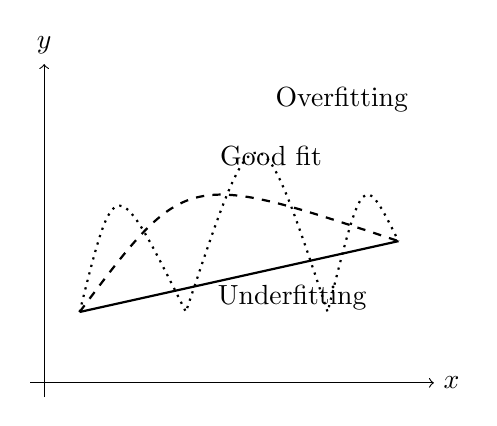
\begin{tikzpicture}[scale=0.9]
  % Axes
  \draw[->] (-0.2,0) -- (5.5,0) node[right] {$x$};
  \draw[->] (0,-0.2) -- (0,4.5) node[above] {$y$};

  % Underfitting
  \draw[thick] (0.5,1) -- (5,2);
  \node at (3.5,1.2) {Underfitting};

  % Good fit
  \draw[thick, dashed] (0.5,1) .. controls (2,3) .. (5,2);
  \node at (3.2,3.2) {Good fit};

  % Overfitting
  \draw[thick, dotted]
    (0.5,1) .. controls (1,3) .. (2,1)
    .. controls (3,4) .. (4,1)
    .. controls (4.5,3) .. (5,2);
  \node at (4.2,4) {Overfitting};
\end{tikzpicture}
\caption{Conceptual illustration of underfitting, good fitting, and overfitting}
\label{fig:overunderfit}
\end{figure}

The visualization highlights how model complexity affects learning behavior.
An underfitted model fails to capture the structure of the data, while an
overfitted model introduces unnecessary oscillations that correspond to noise
rather than meaningful patterns.

\section{Prevention and Mitigation Strategies}
\label{sec:prevention}

Several techniques can be used to reduce underfitting and overfitting in machine
learning models. To address underfitting, one may increase model complexity,
introduce additional relevant features, or allow the model to train for more
epochs. Feature engineering and nonlinear transformations are also common
approaches.

Overfitting can be mitigated through regularization techniques such as L1 and L2
penalties, which constrain model parameters and discourage overly complex
solutions. Early stopping is another effective method, where training is halted
once validation performance begins to degrade. Cross-validation is widely used to
estimate generalization performance and guide model selection.

In practice, selecting an appropriate model requires experimentation and careful
evaluation using separate training, validation, and test datasets.

\section{Conclusion}
\label{sec:conclusion}

This paper discussed the key differences between overfitting and underfitting in
machine learning. Both issues arise from an imbalance between model complexity and
available data. Understanding the bias--variance trade-off is essential for
building models that generalize well to unseen data.

Future work may explore automated model selection techniques and advanced
regularization methods to further improve generalization performance.

This document is formatted using the \texttt{fhjpaper} class provided by FH JOANNEUM
\citep{fhj-script}.

\printbibliography

\end{document}
